% Setup - do not change
\documentclass[11pt]{article}
\usepackage[top=0.9in, left=0.9in, bottom=0.9in, right=0.9in]{geometry} 
\usepackage{parskip}

\usepackage[english]{babel}
\usepackage[utf8]{inputenc}
\usepackage{amsmath,amsthm,amssymb,graphicx,pdfpages,lipsum,hyperref}
\usepackage[none]{hyphenat}
\usepackage{csquotes}

\usepackage{caption}
\usepackage{subcaption}
\usepackage{float}
\usepackage{amsmath}

\setlength\parindent{0pt}
%%%%%%%%%%%%%%%%%%%%%%%%%%%%%%%%%%%%%%%%%%%%%%%%%%%%%%%%%%%%%%%%%%%
% add other packages here if required

%% Bibliography are specified in this file. You can also choose inline bib style if you want to. But make sure your citation style is consistent (and proper)
% For more details on citation: https://library.unimelb.edu.au/recite
\usepackage[sorting = none]{biblatex}
\addbibresource{references.bib}

%%%%%%%%%%%%%%%%%%%%%%%%%%%%%%%%%%%%%%%%%%%%%%%%%%%%%%%%%%%%%%%%%%% the '%' symbol denotes comments

% Begin document creation
% DELETE THE \lipsum PLACEHOLDERS WHEN YOU BEGIN
\title{\textbf{Predicting Features that Impact the Profit of Yellow Taxi Drivers in NYC}}
\author{
Subin Seol \\
Student ID: 1086852 \\
%% Replace the link with your github repo
% 1. Remember to escape underscore (\_) in the link.
% 2. Remember to include the commit you want to submit in the link
\href{https://github.com/MAST30034-Applied-Data-Science/mast30034-project-1-subinai}{Github repo with commit}
}

\begin{document}
\maketitle

\section{Introduction}
% Link to a 30 min tutorial if you require revision: https://www.overleaf.com/learn/latex/Learn_LaTeX_in_30_minutes

In New York City, an iconic yellow taxis play an vital component in daily transportation. Navigating through complex cityscape, the profit of the taxi drivers is influenced by multiple factors. This project \textbf{aims to explore New York City Taxi and Limousine Service Trip Record Data, specifically yellow taxi in January, April, July and October in the year 2022 to identify key elements impacting a taxi driver's profit.} By delving into these essential aspects, the goal of this project is to establish a comprehensive strategy that boosts profitability, deepening our insights into New York's urban transportation economy.

\subsection{TLC Yellow Taxi Data}

The Yellow Taxi data given by the Taxi and Limousine Commission (TLC)\cite{2022sensorreading} provides numerous attributes that are relevant to a single trip. Each data set has more than 10 million rows and 19 columns within the designated month which include pick-up and drop-off time, trip distance, fare amount and etc. Considering the effect of pandemic and lockdown which caused a severe restriction in the lives of the residents in New York City, trip records prior to 2021 may not accurately mirror the current demand dynamics. Consequently, we've chosen to utilise the most recent data set, spanning from January 2022 to October 2022, as the foundation for our modeling and analysis. Given that the trip data wasn't officially curated by the TLC, its authenticity isn't assured. As such, the preprocessing becomes pivotal to ensure data reliability and accuracy.

\subsection{NOAA Weather Data}
The Weather data from the National Oceanic and Atmospheric (NOAA)\cite{2022sensorlocation} offers a detailed perspective on weather patterns in metric unit, complementing our analysis of factors affecting taxi profitability. Comprising roughly 300 rows and 44 columns, it encapsulates weather conditions recorded at New York City Central Park from January to October 2022. This data provides comprehensive metrics, from air temperature and snowfall to precipitation, and average wind speeds. For the sake of our analysis, we operate under the assumption that the weather conditions recorded at this station are representative of the broader New York City area.


% You can have \section{}, \subsection{}, and \subsubsection{}, \section*{}, \subsection*{}, and \subsubsection*{}
\section{Preprocessing}
\subsection{TLC Yellow Taxi Data}
\begin{enumerate}
    \item All the records with missing values were removed and NaN values were converted to 0.
    \item 0 or negative trip distance and passenger count were removed.
    \item Fare amount less than the minimum fare amount (2.5) were removed.
    \item Only cash and card payment were kept in the record as other payment types.
    \item The data types of all attributes were converted correspondingly.
    \item The “trip duration” (in minutes) was created by subtracting “tpep dropoff datetime” from “tpep pickup datetime”.
    \item "Hour", "date", and "day" were extracted from “tpep dropoff datetime” from “tpep pickup datetime”.
    \item Records that have a pick-up time and drop off time outside the range of designated months (January, April, July and October) were removed.
    \item Trip duration longer than 150 (minutes) and less than 1 were removed. Maximum total amount after some preprocessing steps was USD 159.85, fare amount being USD 114.5, travelled for 120.6 minutes. Maximum trip duration, on the other hand, was 5949.95 mins with total amount being USD 63.1. Unreasonably long trip duration that did not match the fare and total amount were disregarded from the data.
    \item Outliers were removed according to the boxplots (see Figure 1a). 
    \item Trip distance and duration with 0 values were replaced with small number, 0.00001.
\end{enumerate}



\subsubsection{Outlier Detection}
After filtering out data that contradicts common understanding, numerous improbable records still persist, as evidenced by the subsequent boxplots of Amount paid which includes fare, tolls and tip amount and the trip distance (refer to Figure 1). Trip records where the trip distance or amounts exceed thrice the Interquartile Range (IQR) are removed to prevent any extreme observations from influencing the evaluation of the model. 

\begin{figure}[H]
    \centering 
     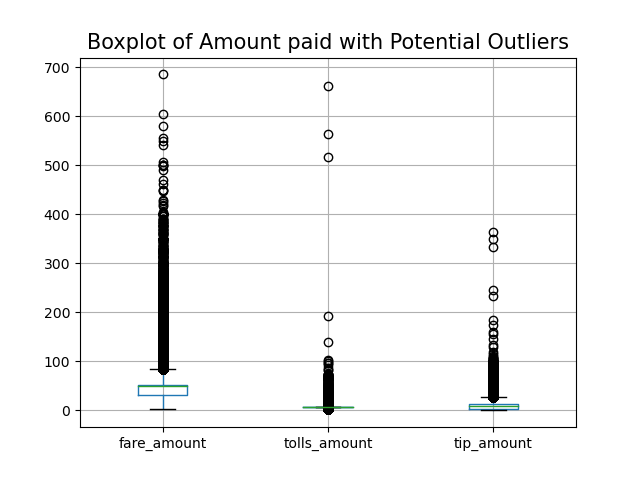
\includegraphics[width=0.4\textwidth]{plots/boxplot of amount paid.png}
     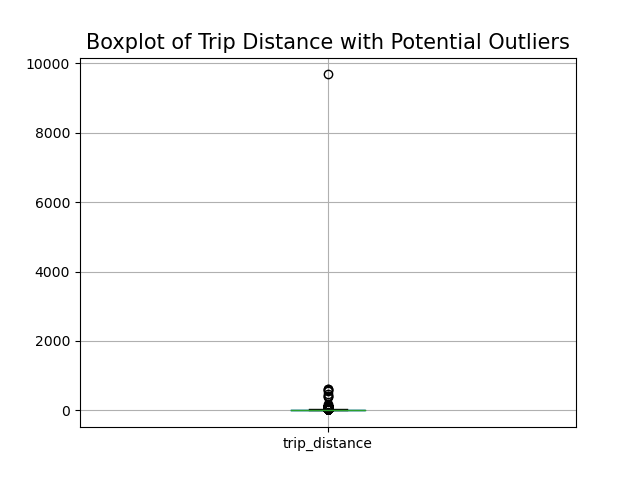
\includegraphics[width=0.4\textwidth]{plots/boxplot of trip distance.png}
     \caption{Boxplot of Amount Paid and Trip Distance with Outliers}
\end{figure}

Upon purging these outliers and replotting the box plot, it's observed that the amounts exhibit a near-normal distribution, with a slight skew to the right (refer to Figure 2).

\begin{figure}[H]
    \centering 
     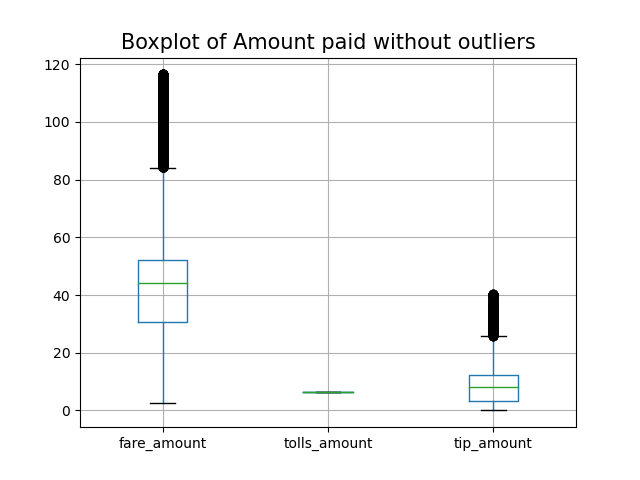
\includegraphics[width=0.4\textwidth]{plots/boxplot of amount paid without outliers.png}
     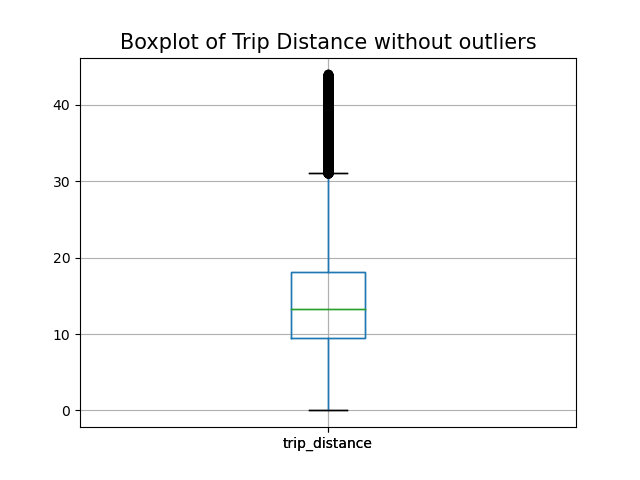
\includegraphics[width=0.4\textwidth]{plots/boxplot of trip distance without outliers.png}
     \caption{Boxplot Amount Paid and Trip Distance without Outliers}
\end{figure}

\subsection{NOAA Weather Data}
\begin{enumerate} 
    \item The data types of all attributes were converted correspondingly.
    \item Average temperature was adding by subtracting TMAX and TMIN and dividing it by 2.
    \item All NaN values were replaced by 0.
    \item Irrelevant column was removed.
    \item A new attribute called "Bad Weather" was created as a binary value to identify weather type either snowing or raining as identified by WT**.
\end{enumerate} 

\section{Analysis and Geospatial Visualisation}
The "profitability" of the Yellow Taxi drivers is mostly based on the fare amount and the tip paid by the passenger. Taxi fares are charged by the time and the travelled distance, but there are other crucial components such as traffic jams during rush hour that can impact the amount earned. 

\begin{figure}[H]
    % change the scale multiplier to make the figures smaller or larger
    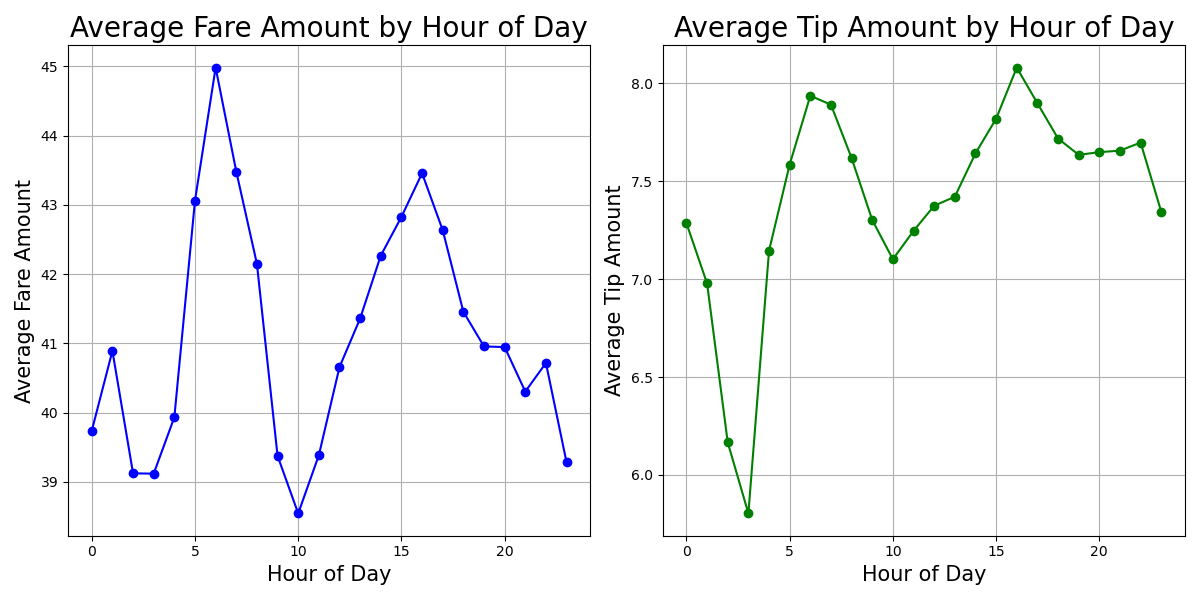
\includegraphics[width=0.6\textwidth]{plots/Avg amount by hour of day.png}
    % this ensures your figures are centered where possible
    \centering
    \caption{Average Fare and Tip Amount received by Hour of the Day} % refer to this image as (Figure 1)
\end{figure}
In Figure 3, it is certain that there is a pattern showing which time period taxi drivers benefit the most. The early morning hours, particularly around 5 AM, show a notable spike in both fare and tip amounts. This increase might be a result of limited taxi availability during these hours, which can lead to elevated fares. Another factor could be early morning airport commutes, as passengers typically prefer flights at the start of the day, and the extended journey to the airport can command higher charges. A distinct increase in earnings, particularly between 6 PM and 9 PM can be attributed to the evening rush, with people returning from work and a heightened overall demand. While fare and tip amount seem to have a similar pattern of peak profit time zone, tip appears steadier. This indicates that while the fare for a trip might differ based on elements like demand and travel length, the proportion of tips passengers offer tends to be more uniform.

\begin{figure}[H]
    % change the scale multiplier to make the figures smaller or larger
    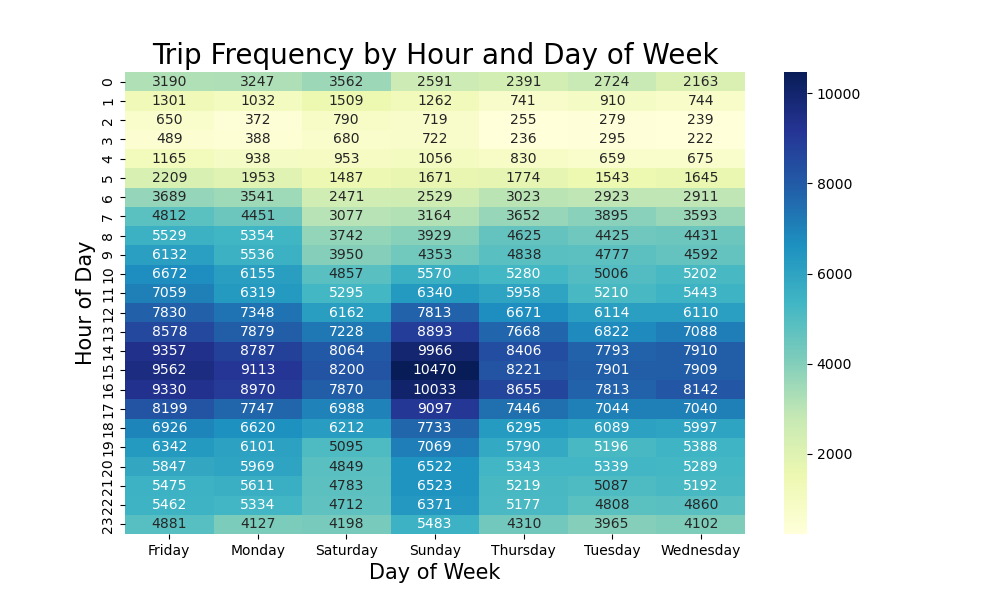
\includegraphics[width=0.8\textwidth]{plots/trip frequency by hour and day of week.png}
    % this ensures your figures are centered where possible
    \centering
    \caption{Trip Frequency by hour and day of week} % refer to this image as (Figure 1)
\end{figure}

Undoubtedly, the frequency of trips stands as a pivotal determinant in shaping profitability. While Figure 3 established the significance of taxi demand that increases the fare amount, Figure 4 shows a high demand in the afternoon (12pm to 5pm) driven by office commuters, tourists, and regular city activities. Furthermore, during the weekends, demand begins to escalate later than the  weekdays especially on Sunday, sustaining its momentum until late evening. This trend can be attributed to the late-night activities.

\begin{figure}[H]
    % change the scale multiplier to make the figures smaller or larger
    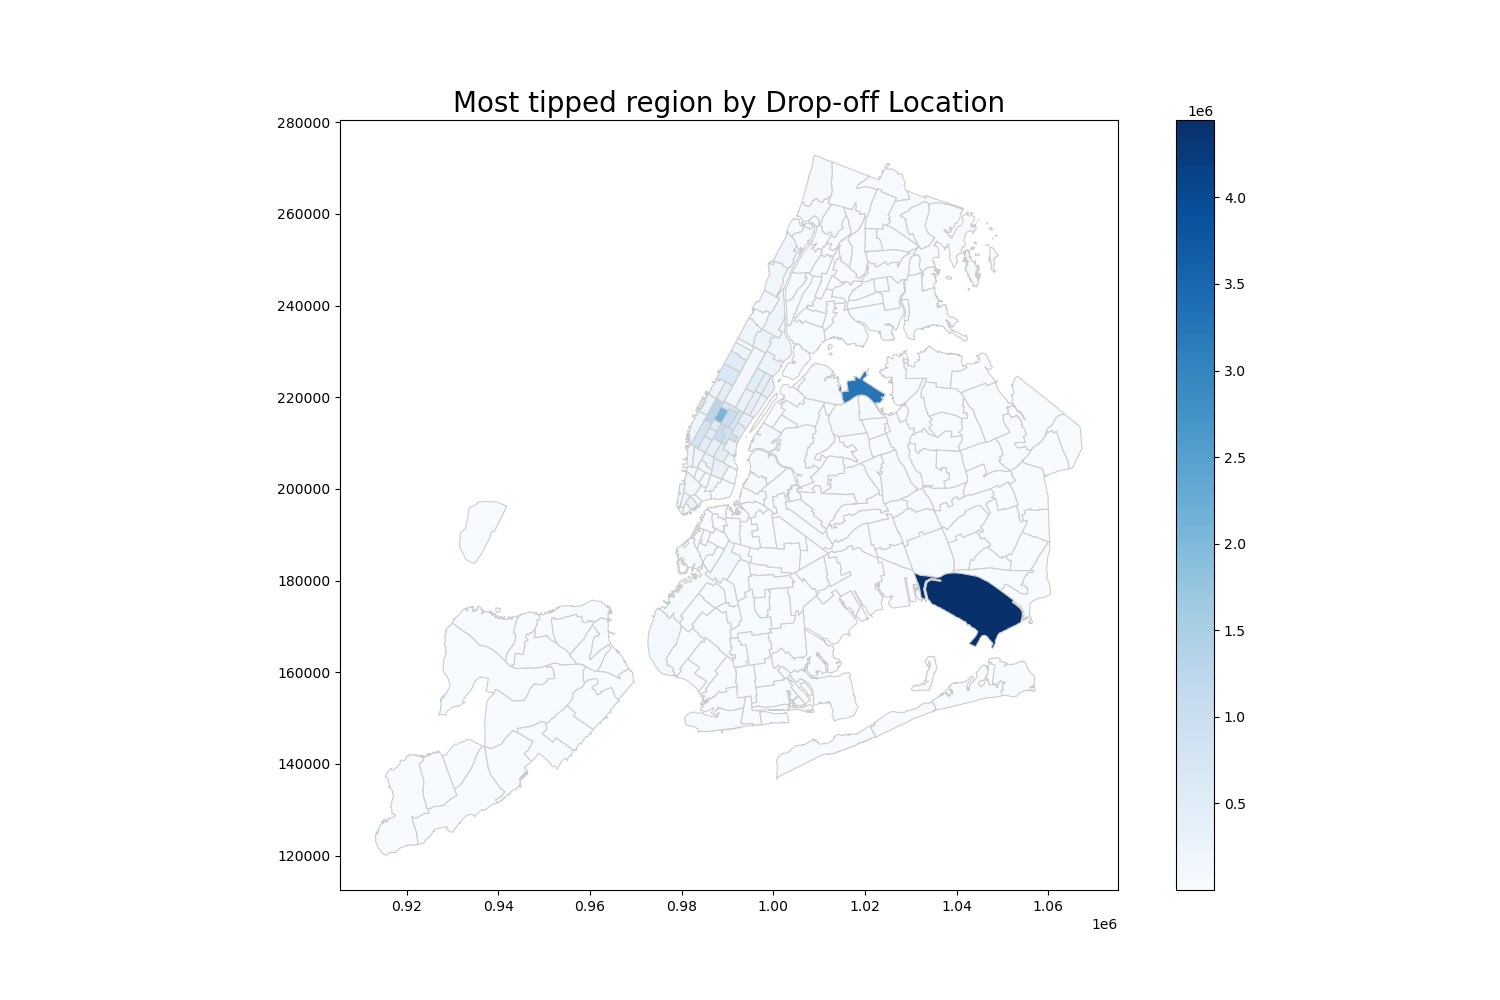
\includegraphics[width=0.9\textwidth]{plots/most tip by drop-off location.png}
    % this ensures your figures are centered where possible
    \centering
    \caption{Most Tipped Area by Drop-off Location} % refer to this image as (Figure 1)
\end{figure}

Figure 5 is a geographic visualisation of most tip received location. Key transit hubs like JFK and LaGuardia airports are evident high-tipping areas. The extended journey lengths to these destinations, combined with set airport tariffs and the appreciative tipping behavior of travelers - possibly for the added service convenience and luggage assistance - contribute to this trend. Additionally, Manhattan, being the Financial District stands out as a brimming area with businesses, and tourist magnets, naturally drawing higher fares, leading to increased tips.


\begin{figure}[H]
    % change the scale multiplier to make the figures smaller or larger
    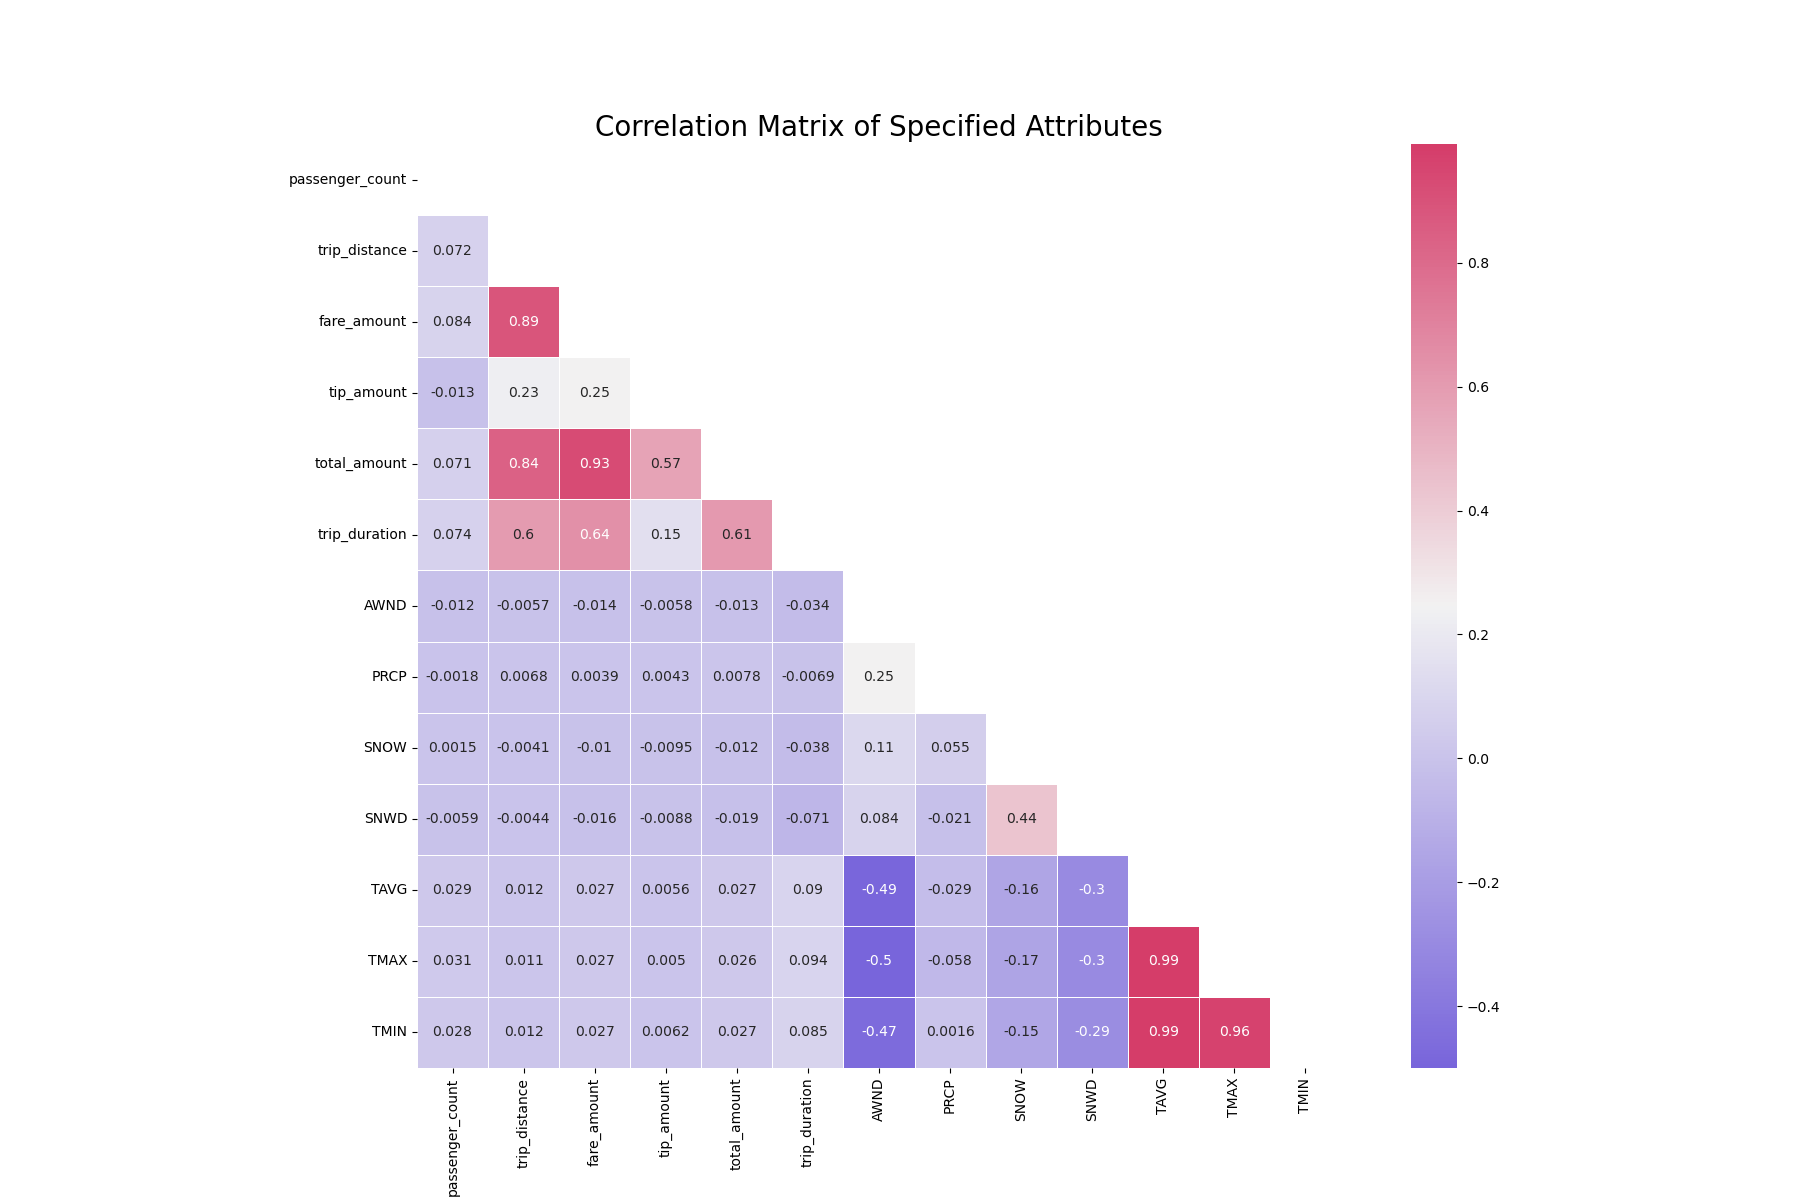
\includegraphics[width=0.95\textwidth]{plots/correlation matrix.png}
    % this ensures your figures are centered where possible
    \centering
    \caption{Some caption} % refer to this image as (Figure 1)
\end{figure}

To assess the impact of the weather on the profit of taxi drivers, the correlation between each attributes are computed in Figure 6. Snowfall, snow depth and wind speed labelled as "SNOW", "SNWD" and "AWND" respectively are negatively correlated to passenger count, trip distance, fare amount and trip duration. While the observed correlations are not pronounced, it remains essential to explore the nuanced influence of weather conditions on a taxi driver's profitability.

\section{Modelling}
\subsection{Profit Label}

The average profit per distance and duration in minute is calculated as:
  \[
    \text{Avg Profit} = \frac{\frac{\text{Fare Amount} + \text{Tip Amount}}{\text{Trip Distance}} + \frac{\text{Fare Amount} + \text{Tip Amount}}{\text{Trip Duration}}} {2}
  \]

Since the statistical models explored in this project are used for categorical values, we create a new variable called profit label by converting the average profit to binary output. We labelled each instance with 0 and 1:
\begin{itemize}
        \item[*] 0: When the average profit is less the median average profit, which means that the average fare and tip amount per distance and duration is below 50\% quantile.
        \item[*] 1: When the average profit is greater the median average profit, which means that the average fare and tip amount per distance and duration is above 50\% quantile.
\end{itemize}

\subsection{Train and Test Data}
Features of train and test data sets focused on the variables that are relevant to the profit level which include trip distance, trip duration, passenger count, temperatures, and weather conditions. Features are then standardised, divided into train and test with by test size 0.2.

\subsection{Random Forest Classifier}
The Random Forest Classifier (RFC) is a potent machine learning technique employed in this study. It functions by creating a 'forest' of multiple decision trees during the training phase, delivering the most frequent class label from each tree for new data. The underlying concept of RFC is to combine the outcomes of multiple decision trees, ensuring a prediction that is more precise and stable than a singular tree. Every tree within this forest emerges from a dataset obtained with repetition. Additionally, while creating branches in these trees, only a random selection of features is taken into account. This strategy ensures that the trees are not highly correlated, leading to a decrease in the ensemble's overall variance.

From the given data, the optimal configuration for the Random Forest Classifier after hyperparameter tuning is: n\_estimators: 500, min\_samples\_split: 5,
min\_samples\_leaf: 1, max\_features: 'log2', max\_depth: 10, bootstrap: False. 

Comparing the base model and the RFC with best parameters, the overall accuracy progressed from 0.72 to 0.75 with the improvement of of 4.849\%. The optimum model predicted that 88\% of the instances correctly identified as 'low profit' and 69\% correctly labelled as 'high profit'. High recall for class 1 (92\%) established that out of all 'high profit' labels, the classifier was able to apprehend a large majority of them, suggesting that false negatives (where actual high profit are predicted as low profit) are low. RFC model performed quite well by capturing positive instances of class 1 with the recall being 0.92, only missing the 8\% of them, but this also means that when it comes to predicting 'high profit', it is less reliable than predicting class 0 as suggested by lower precision score for class 1 compared to 0. 

Using the RFC model, now we created a feature importance plot to observe which feature impacted the profit level the most. 

\begin{figure}[H]
    % change the scale multiplier to make the figures smaller or larger
    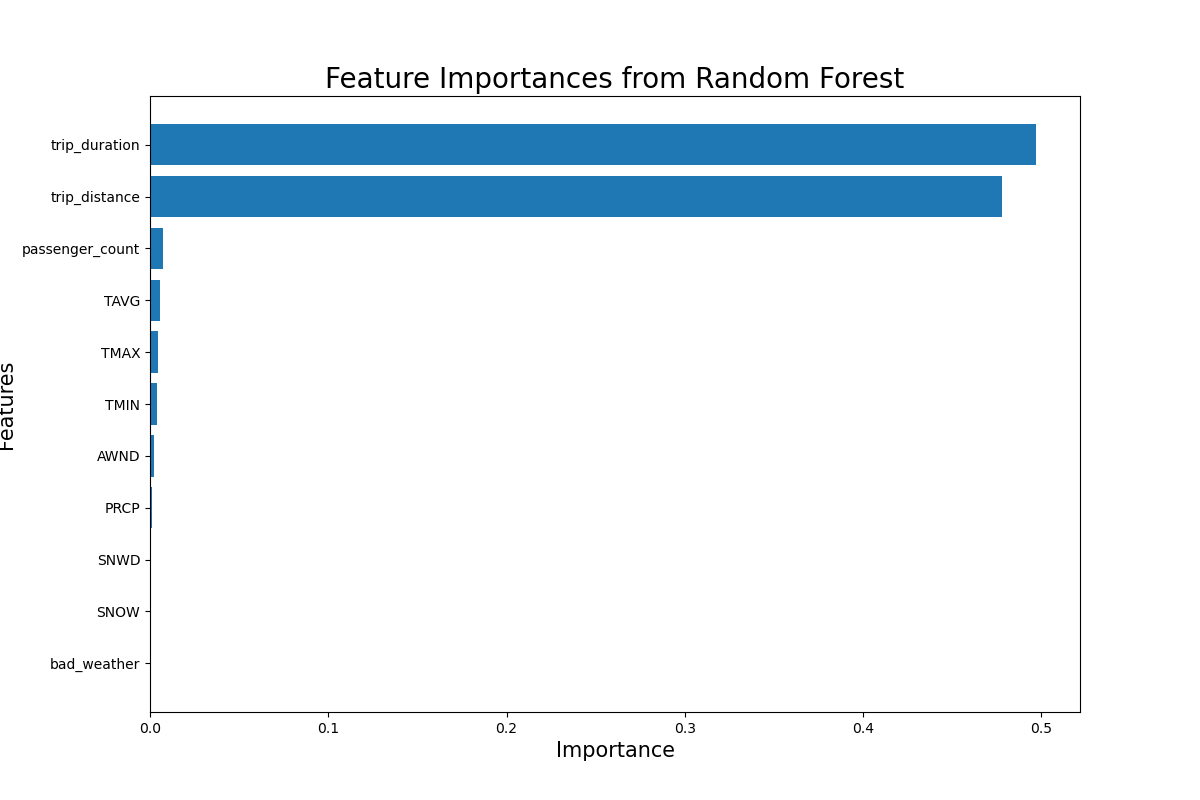
\includegraphics[width=0.45\textwidth]{plots/Feature importances from RFC.png}
    % this ensures your figures are centered where possible
    \centering
    \caption{Feature Importance from Random Forest Classifier} % refer to this image as (Figure 1)
\end{figure}

Figure 7 shows that trip duration and distance affects the profit of taxi drivers which is the obvious result as the fare amount is high dependent on the time and distance of the trip. Passenger count and average temperature also appear to have a small impact on the profit. High number of passengers might share a ride to a further destination and separate fare among themselves or there is a possibility of tipping behaviour. Additionally, the demand for taxi services can be influenced by the day's average temperature, with extremely cold or hot days possibly pushing people to opt for taxis over walking or other transportation modes.

\subsection{Logistic Regression}
Logistic Regression is a statistical model that is widely used for binary classification problems. It predicts the probability of an instance belonging to a default class, which can be converted into a binary outcome via a threshold.

The confusion matrix of the model showed a very balanced performance in predicting both class 0 and 1 with a fair score of precision, accuracy and recall of 70\%, therefore demonstrating relatively good prediction.  

The evaluation of Logistic Regression is less accurate compared to the RFC model and this may be due to the their complexity and the performance of the model itself. RFC is generally more complex which can capture non-linear correlations while LR assumes a linearity of the variables. Furthermore, with hyperparameter tuning, Random Forest is less prone to overfitting despite the size of the given data, thus based on the nature of our data in this project, RFC outperforms in predicting two classes of profit level. 

\section{Discussion and Recommendations}
Visualisations and statistical modelling using Random Forest Classifier and Logistic Regression shows a clear pattern of relationship between the data features and the taxi driver's profit. One of the strategic approach to maximise the profit of taxi drivers is considering the time for the heightened demand notably during early mornings, around 5 AM, and during the evening rush between 6 PM and 9 PM. By aligning their operations to cater these peak hours, drivers would significantly boost their earnings. Moreover, weather conditions also correlates to the taxi demand as validated by studies like Lepage and Morency (2021)\cite{Lepage:2022}. Extreme temperatures or bad weathers like rain and snow can either lead to amplifying taxi demand to avoid walking. As such, paying a close attention on the weather forecast and adapting accordingly can be a competitive advantage. Geospatial data analysis also points to specific locations like JFK and LaGuardia airports, as prime locations for higher tips. Taxi drivers can strategically focus on these areas, especially during the early morning, to tap into this lucrative passengers. Aside from daily patterns of time and weather, major city events such as concerts and sports games can trigger a surge in taxi demand.  Staying updated with the city's event roster allows drivers to be in the right place at the right time, maximising their earning potential.

\section{Conclusion}
Our analysis highlighted key drivers of taxi driver profitability, including peak operating hours, weather impacts, and strategic location positioning. As urban landscapes evolve, especially post-pandemic, taxi drivers and industry stakeholders must adapt to these findings to retain a competitive benefit in the transport sector. Since this study was only based on the binary output, Random Forest Regressor or Linear regression can be used to utlise continuous variable of profit and specifically predict how much can taxi drivers earn depending on the attributes.

\clearpage

% BEGIN REFERENCES SECTION
\printbibliography

\end{document}